\documentclass[12pt]{article}
\usepackage[utf8]{inputenc}
% Deutsch: https://de.overleaf.com/learn/German
% "`	Left double quotes
% "'	Right double quotes
\usepackage[T1]{fontenc}
\usepackage[ngerman]{babel}
\usepackage{csquotes}

\usepackage{xcolor}
\usepackage{listings}

\usepackage{tikz}
\usetikzlibrary{positioning,automata}

\usepackage[acronym,nonumberlist]{glossaries}
\usepackage{acronym}

% documentation: https://ctan.kako-dev.de/macros/latex/contrib/biblatex/doc/biblatex.pdf
\usepackage[backend=biber,style=numeric,sorting=ynt]{biblatex}
\addbibresource{references.bib}

% um Grafiken einzubinden, {Angabe des Pfades der Bilder}
\usepackage{float}
\usepackage{graphicx}
\graphicspath{ {images/} }
% Nützliches Online Tool zur Tabellengenerierung: TablesGenerator.com 

% zur korreten Platzierung der Bilder im Titelblatt
\usepackage{chngpage}
\usepackage{calc}
\usepackage{geometry}

% Automatisches Generieren von Hyperlinks bei Verweisen (ref / cite)
\usepackage{hyperref}
\hypersetup{
  colorlinks   = true,    % Colours links instead of ugly boxes
  urlcolor     = blue,    % Colour for external hyperlinks
  linkcolor    = black,    % Colour of internal links
  citecolor    = red      % Colour of citations
}

% Infos über Dokument
\title{Progressive Web Apps}
\author{Sebastian Pötter}
\date{\today}

\begin{document}

    \newgeometry{top=2cm,bottom=2cm}

\begin{titlepage}
    
    \begin{figure}[t]
        \begin{adjustwidth}{-\oddsidemargin-1in}{-\rightmargin}
            \centering
            
\includegraphics[width=\paperwidth]{banner_top}
        \end{adjustwidth}
    \end{figure}

    \begin{flushleft}
        \vspace*{1cm}
        \Huge
        \textbf{Progressive Web Apps}
        
        \vspace{0.5cm}
        \LARGE
        Notiz-App
        
        \vspace{1.5cm}
        \textbf{Sebastian Pötter}
        
        \vspace{0.5cm}
        \large
        Jahrgang: 20INM
        
        \vspace{0.5cm}
        im Studiengang\\
        Informatik Master
        
    \end{flushleft}        

    \vspace{0.5cm}
    \begin{flushright}
        Progressive Web Applications (C367)\\
        Prof. Michael Frank\\
        \vspace{0.5cm}
        \today
    \end{flushright}    
    
    \begin{figure}[b]
        \begin{adjustwidth}{-\oddsidemargin-1in}{-\rightmargin}
            \centering
        \end{adjustwidth}
    \end{figure}

\end{titlepage}

\restoregeometry
    \newpage
    
    \pagenumbering{roman}

    \tableofcontents
    
    \newpage
        
    \addcontentsline{toc}{section}{Abkürzungsverzeichnis}  
    \section*{Abkürzungsverzeichnis}
        \begin{acronym}
            \acro {PWA} {Progressive Web Apps}
            \acro {CSS} {Cascading Style Sheets}
            \acro {HTML} {HyperText Markup Language}
            \acro {PHP} {Hypertext Preprocessor}
            \acro {SQL} {Structured Query Language}
            \acro {SASS} {Syntactically Awesome Stylesheets}
            \acro {MVC} {Model, View, Controll}
            \acro {CORS} {Cross-Origin Resource Sharing}
            \acro {URL} {Uniform Resource Locator}
            \acro {REST} {Representational State Transfer}
            \acro {JSON} {JavaScript Object Notation}
            \acro {NPM} {Node Package Manager}
            \acro {XSS} {Cross Site Scripting}
        \end{acronym}
    
    \newpage
    
    \pagenumbering{arabic}
    
    \section{Einleitung}
    
Im Rahmen des Moduls 'Progressive Web Apps' soll eine Webanwendung entwickelt werden. Die Art von Webanwendung kann, nachdem sie einmal geladen wurde, offline weiterhin benutzt werden. Zusätzlich biete sich die Möglichkeit, diese Anwendung auf dem Gerät zu installieren. Hierfür ist das so genannte 'Webmanifest' und der 'Service Worker' zuständig. Im 'Webmanifest' befinden sich die nötigen Informationen der Ressourcen. Ein 'Service Worker' ist ein Skript, das imHintergrund des Browsers ausgeführt wird.  Heute gehören dazu bereits Funktionen wie Push-Benachrichtigungen und Hintergrundsynchronisation, sowie Installationsfunktionen. PWA's lassen sich normalerweise auch im Browser installieren, oder auf dem SmartPhone als pseudo-App hinzufügen. 
    
    \section{Architektur}
    
Das folgende Kapitel handelt von der Architektur der Webandwendung und des Servers samt API. Von allen Frameworks und Bibliotheken wurden die aktuellsten Versionen genommen um diese besser kennen zu lernen. 

        \subsection{Frameworks und Bibliotheken}
            Folgende Bibliotheken und Frameworks wurden für diese Webanwendung benutzt:
            \begin{itemize}
                \item Bootrap 5
                \item Jquery 3.6
                \item Popper 2
                \item Angular 12.1.1
                \item CakePHP 4
                \item FontAwesome 5
                \item MariaDB 10.5.11
            \end{itemize}
            Verwendete 'Programmiersprachen':
            \begin{itemize}
                \item PHP 7.4
                \item Typescript 4.2.4
                \item MySQL 8.0
                \item SASS (CSS3)
                \item HTML 5
            \end{itemize}
        
        \subsection{Cake PHP Server}

CakePHP wurde entwickelt, um gängige Webentwicklungsaufgaben einfach und leicht zu machen. Durch die Bereitstellung einer All-in-One-Toolbox für den Einstieg arbeiten die verschiedenen Teile von CakePHP gut zusammen oder separat. CakePHP ist ein Open-Source-Web-Framework. Es folgt dem Model-View-Controller (MVC)-Ansatz und ist in PHP geschrieben. Die Abbildung \ref{fig:architecture-cakephp} zeigt den Aufbau einer CakePHP Anfrage.

CakePHP verwendet bekannte Software-Engineering-Konzepte und Software-Design-Patterns, wie zum Beispiel Konventionen über Konfiguration, Model-View-Controller, Active Record, Association Data Mapping und Frontend-Controller. Plugins ermöglichen es Entwicklern, Kombinationen von Controllern, Models, Views und anderen Klassen für die Wiederverwendung in mehreren Anwendungen und durch andere Entwickler zu verpacken. 
\begin{figure}[h!]
    \caption{CakePHP Aufbau}
    \centering
    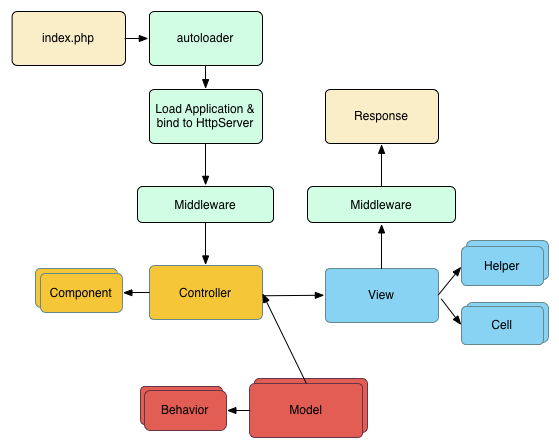
\includegraphics[width=0.7\textwidth]{architecture-cakephp.png}
    \text{\tiny \url{https://book.cakephp.org/4/en/_images/typical-cake-request.png}}
    \label{fig:architecture-cakephp}
\end{figure}
        
        \subsection{Angular Webandwendung}

Angular ist ein Anwendungsdesign-Framework und eine Entwicklungsplattform für die Erstellung effizienter und anspruchsvoller Single-Page-Apps. JavaScript ist die am häufigsten verwendete Client-seitige Skriptsprache. Sie wird in HTML-Dokumente geschrieben, um Interaktionen mit Webseiten auf viele einzigartige Arten zu ermöglichen. Als relativ einfach zu erlernende Sprache mit weit verbreiteter Unterstützung ist sie gut geeignet, um moderne Anwendungen zu entwickeln. Heutzutage gibt es eine Vielzahl von Frameworks und Bibliotheken, die alternative Lösungen bieten. In Bezug auf die Front-End-Webentwicklung löst Angular viele, wenn nicht sogar alle Probleme, mit denen Entwickler konfrontiert werden, wenn sie JavaScript ohne Bibliothek verwenden. Die Abbildung \ref{fig:architecture-angular} zeigt den Aufbau einer Angular Anwendung. 

Zusätzlich ist es möglich Angular in Typescript zu Programmieren. TypeScript ist eine Open-Source-Sprache, die auf JavaScript aufbaut, indem sie statische Typisierung hinzufügt.
\begin{figure}[h!]
    \caption{Angular Aufbau}
    \centering
    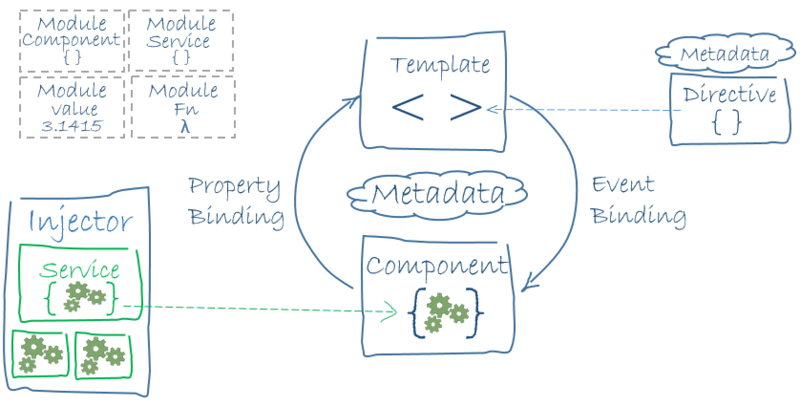
\includegraphics[width=0.8\textwidth]{architecture-angular.png}
    \text{\tiny \url{https://en.wikipedia.org/wiki/File:Architecture_of_an_Angular_2_application.png}}
    \label{fig:architecture-angular}
\end{figure}

    \section{Dokumentation}

Dieses Kapitel soll sich mit der Dokumentation des Quellcodes befassen. Dabei wird sowohl der Logische Aufbau als auch der Sourcecode selbst des Projektes vorgestellt und erklärt. 

        \subsection{Ordnerstruktur}

Das Projekt ist in 2 Hauptordner unterteilt. Der Ordner 'app' und 'note-app'. Der 'app' Ordner beinhaltet den PHP Server mit dem Framework 'CakePHP'. Die Angular Webanwendung befindet sich im 'note-app'. Im folgenden wird die Ordnerstruktur des Servers vorgestellt (siehe Abb. \ref{fig:path-php}).
\begin{figure}[h!]
    \caption{CakePHP Ordnerstruktur}
    \centering
    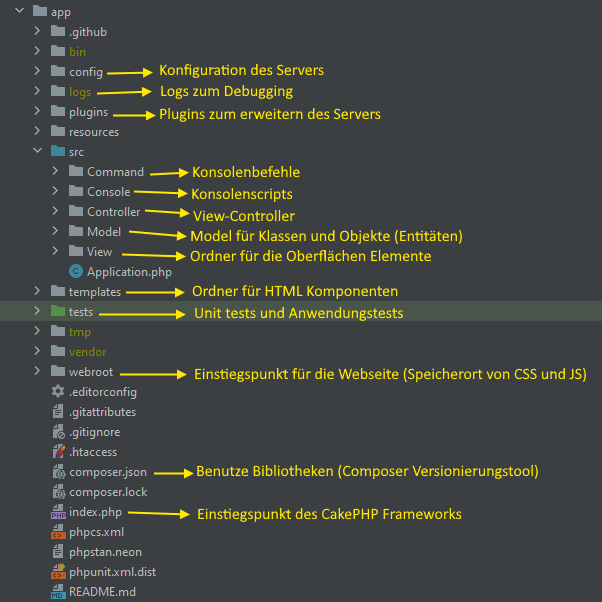
\includegraphics[width=0.8\textwidth]{cakephp-paths.png}
    \label{fig:path-php}
\end{figure}

Darauf folgend auch die Ordnerstruktur der Angular App (siehe Abb. \ref{fig:path-angular}) mit Erklärung zu bestimmten Dateien und speziellen Ordnern.
\begin{figure}[h!]
    \caption{Angular Ordnerstruktur}
    \centering
    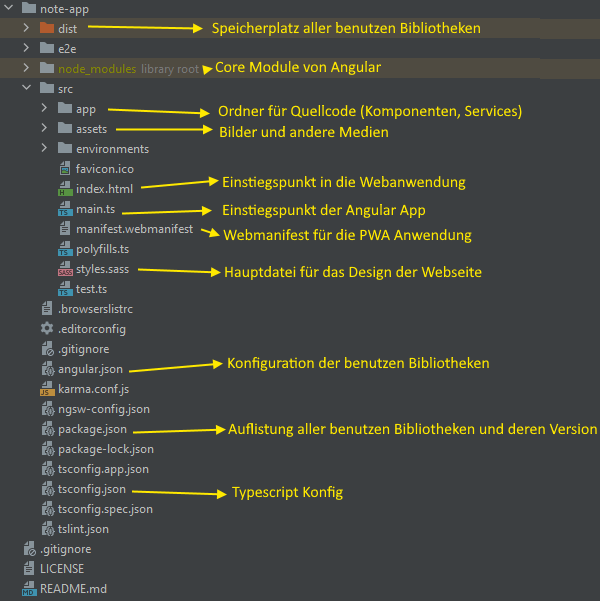
\includegraphics[width=0.8\textwidth]{angular-paths.png}
    \label{fig:path-angular}
\end{figure}


        \subsection{Server}

Der Server verwendet die aktuellste CakePHP 4 Version mit allen Standard-Plugins, wie zum Beispiel 'Migrations', was für die Datenbank Versionierung benutzt wird. 

            \subsubsection{MVC Aufbau}
            
Der Server ist einfach aufgebaut. Es gibt zwei Modelle: das User-model ('src/Model/Table/UsersTable.php') und das Note-model ('src/Model/Table/NotesTable.php'). Diese beinhalten die Information der User/Note Klasse und die Strukturinformation der Datenbank sowie die Verlinkung untereinander. Die Note Tabelle verweist mit dem Sekundärschlüssel User\_id auf die Tabelle User. Damit ist eine 1:n Beziehung hergestellt, sodass ein User mehrere Notizen haben kann. Jedes Model hat Entitäten, vergleichbar mit einem Objekt einer Klasse. Diese Entitäten können noch Eigenschaften und weitere Funktionen besitzen. Die die User-Entität ('src/Model/Entity/User.php') besitzt darüber hinaus die Funktion zur verschlüsselung des Passwortes. Die Note-Entität ('src/Model/Entity/Note.php') enthält die Funktion zum Ver-Entschlüsseln des Notizen-Inhalts. Die Entitäten beschreiben zusätzlich das Verhalten aller Eigenschaften, was beispielsweise dazu führt, dass der SALT des Users nicht nach außen weitergegeben wird sondern privat ist (anstelle von public).

Der einzige Kontroller des Servers ist der API Kontroller ('src/Controller/ApiController.php'). Dieser Erbt vom Hauptkontroller der CakePHP-Bibliothek und benutzt zusätzlich noch einen selbst geschriebenen Login-Komponente ('src/Controller/Component/LoginComponent.php'), welcher den Authentifizierungsvorgang bereitstellt. Die 'initialize' Methode im Kontroller ist für das Laden aller benötigten Modelle und Komponenten Zuständig. Die 'beforeFilter' Methode wird immer Aufgerufen wenn auf eine Methode des Kontrollers aufgerufen wird, hier wird sie für das Freischalten der CORS-Prüfung benutzt, da dieser Server den CORS-Schutz benötigt. 'Index', 'authenticate', 'register', 'createNote', 'getNotes', 'editNote' und 'deleteNote' sind die Methoden, welche die REST-API Daten zur Verfügung stellen und per URL abgerufen werden können. Die Index-Methode ist hierfür nur zum Test gedacht, da diese alle Notizen lädt um zu zeigen, dass die Datenbankabfrage über die API funtkioniert.

Da der Server nur eine API bieten soll, gibt es kein VIEW-Element. Jede Anfrage an den Server endet mit einer Antwort als JSON Datei. 
            
            \subsubsection{REST API}
        
Wie im vorherigen Kapitel erklärt, besitzt der API-Kontroller alle Funktionen für die REST-API. Um dies besser zu veranschaulichen, wurde mit \url{https://swagger.io} (siehe Abb. \ref{fig:api}) eine Übersicht erstellt. Swagger ist dafür gedacht eine automatisierte Erstellung einer vollständigen API als Server zu erstellen (CakePHP gehört nicht dazu).
\begin{figure}[h!]
    \caption{REST API des Servers}
    \centering
    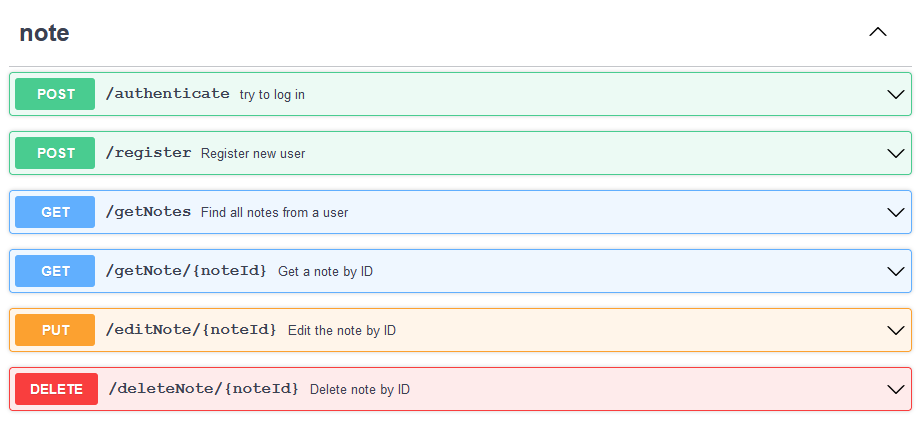
\includegraphics[width=1\textwidth]{api.png}
    \label{fig:api}
\end{figure}

        \subsection{Webanwendung}

Die Webanwendung benutzt NPM um die Angular-Bibliothek zu installieren. NPM ist ein Paketmanager für die Programmiersprache JavaScript und Typescript. Dieses Kapitel beschäftigt sich mit dem Aufbau und der Logik der Webanwendung.

            \subsubsection{Klassen}

Die gesamte Anwendung benutzt nur zwei Klassen, die Note-Klasse ('src/app/notes.ts') und die User-Klasse ('src/app/user.ts'). Diese haben die selbe Eigenschaften wie die Klasse auf dem Server. Note: sie besitzt Name, Titel, Erstellungsdatum, Text und Bearbeitungsdatum und User: Name, Password und Erstellungsdatum.

Die App.module ('src/app/app.module.ts') ist für das Laden des Service Workers zuständig, welcher bereits vorkonfiguriert ist direkt geladen wird. Dieser Service-Worker kümmert sich um das Caching und das installieren als APP. 
            
            \subsubsection{Komponenten}

Die App.Komponent ('src/app/app.component.ts') ist, wie bei anderen Programmiersprache die 'Main Methode', der Haupteinstiegspunkt der Angular Anwendung und besitzt eine Variable die den Titel der Anwendung repräsentiert. Jede Komponente besitzt eine Style Datei (SASS), eine Typescript Datei und eine HTML Datei. Eine Komponente kann in eine andere Komponente verlinkt werden oder auf andere zeigen. Außer der App Komponente werden andere Komponenten in Unterordnern gespeichert. 

Die Notes Komponente ('src/app/notes') kümmert sich um das Laden aller Notizen und listet diese auf. Zusätzlich beinhaltet diese Komponente die Methode zum updaten der Notizen falls die Verbindung wiederhergestellt ist. 

Der Header der Anwendung wird in der Note-header Komponente ('src/app/note-header') erstellt. Da die Anwendung auch Bootstrap 4 benutzt. Bootstrap ist ein Framework für das fluide Darstellen und weiteren Features verantwortlich und nimmt eine Menge anpassungsarbeit ab. Hier wird auch der Titel aus der Hauptkomponente und der Status geladen.

Wenn auf eine Notiz geklickt wird, dann wird die Note-detail Komponente ('src/app/note-detail') geladen, welche für das Anzeigen eines Popups zuständig ist. In diesem Popup wird der Titel und andere Eigenschaften der Notiz geladen, welche es von der Notes Komponente bekommt. Wenn man den Speichern/Lösch-Button drückt, dann wird noch ein Event ausgelöst, welche eine Aktualisierung der Notiz auslöst. Diese Aktualisierung wird im nächsten Kapitel näher erklärt. 

Möchte man eine neue Notiz anlegen, so wird nach dem Klick auf das Plus-Zeichen, die Note-add Komponente ('src/app/note-add') geladen und wieder ein Popup fenster angezeigt. Diese Komponente löst nach dem Klick auf den Speicher-Button ein Event aus, welche auch wieder einen Service benachrichtigen. 

Die Messages Komponente ('src/app/messages') ist für das Anzeigen von Fehlern zuständig und wird von der App.module geladen wird.
        
            \subsubsection{Services}

Der auth.service ('src/app/auth.service.ts') ist für den Authenfizierungsvorgang zuständig. Dieser Service enthält den Login per API. Zusätzlich enthält dieser Service die Information, ob Internet verfügbar ist und ob er User eingeloggt ist. Der Authservice wird von vielen Komponenten und anderen Services benutzt. 

Um die Kommunikation mit dem Server zu gewährleisten wird der Note.service ('src/app/note.service.ts') benutzt. Dieser Service besitzt alle Funktionen, welche die API bereitställt. Es können Notes geladen, erstellt, geändert und gelöscht werden. Da die REST-API ein zustandloses Protokoll ist, wird auch immer der Nutzername und das Passwort mitgesendet, welche auf dem Server überprüft werden. 

Um Daten wie die Notizen zu speichern, wird der local-storage.service ('src/app/local-storage.service.ts') bentzt. Dieser entählt die einfache Funktionen zum add/set/get von Local-Storage Daten bis hin zu komplexeren Synchronisierung Funktionen. GetNotes läd alle verfügbaren Notizen und benutzt hierfür die Get-Methode. AddNote fügt eine neue Notiz den bestehende Notizen hinzu. SetNotes beinhaltet die Synchronisierung, welche später näher erklärt wird. Die deleteNote Methode ist für das Löschen einer einzelnen Notiz zuständig, hierfür wird die ID in local-storage gesucht und dann aus dem Array gelöscht.

Um die Nachrichten wie Fehlermeldungen ordentlich weitezugeben wird der message.service ('src/app/message.service.ts') benutzt, welche die Fehlermeldungen dem Array hinzufügt und dann ein Event für das Anzeigen wirft.

Der remote-managing.service ('src/app/remote-managing.service.ts') ist der Hauptservice für die Kommuniktation zwischen oline/offline Service (also local-storage.service und note.service), in jeder Funktion wird geprüft ob man eingeloggt ist. Wenn der Nutzer online und verifiziert ist, werden die Notizen auf dem Server gespeichert. In jedem Fall werden die Notizen lokal abgeändert, um die Offlinefähigkeit zu gewährleisten. 

        \subsection{Funktionsweise der Synchronisierung}
        
Dieses Kapitel soll sich mit der Funktionalität rund um den Wechseln von Online zu Offline und andersherum beschäftigen. Die Notizen werden immer auf der Lokalen Ebene geändert, besteht jedoch die Verbindung zum Server werden die Notizen auch in der Datenbank gespeichert. Dabei ist es wichtig, dass es nicht zu Merge-Fehlern kommt, weswegen wichtig ist dort eine feste Regel zu definieren. 

Wenn die Anwendung offline arbeitet und dann online geht, gleicht die Anwendung die heruntergeladenen Notizen mit den lokalen ab und prüft welche Version der selben Notiz aktueller ist (last\_edited) und läd danach die aktuellste Version wieder auf den Server. Wird lokal eine neue Notiz erstellt, wird diese auf den Server hochgeladen. Wird eine Notiz lokal gelöscht während man offline ist, muss diese erneut gelöscht werden, wenn man wieder online ist. 
    
    \section{Lernerfahrungen}

Ich habe in diesem Projekt eine Menge in Sachen Webentwicklung und PWA dazugelernt. In diesem Projekt habe ich auch das erste mal sowohl Angular als auch Typescript benutzt, und ich kann mir vorstellen auch weitere Projekt mit diesem Framework zu entwickeln. Zusätzlich konnte ich das erste mal Bootstrap 5 ausprobieren, welche zum jetzigen Zeitpunkt noch eine Beta-version ist. Ich konnte sogar einen Fehler in Bootstrap melden, da die Offcanvas funktion (das ausfahren eines Div-Containers) in der momentanen Bootstrap Version nicht funktioniert.  Zusätzlich konnte ich GitHub Pages mal testen und weiß nun, dass es mit externen Servern nicht sehr gut klar kommt, weil CORS nicht richtig funktionieren und diese als XSS behandelt wird. Es war interessant an dieser Anwendung zu arbeiten und ich versuche diese auch noch weiter zu entwickeln. Auch die Registrierungfunktion funktioniert noch nicht auf der Webanwendung, der Server hat dennoch Funktionen für die Registrierung. Genauso auch die Login-Funktion welche auf der Github Pages nicht mit dem Server verbinden kann.

\end{document}